\section{Appendix}
\begin{figure}
    \centering
    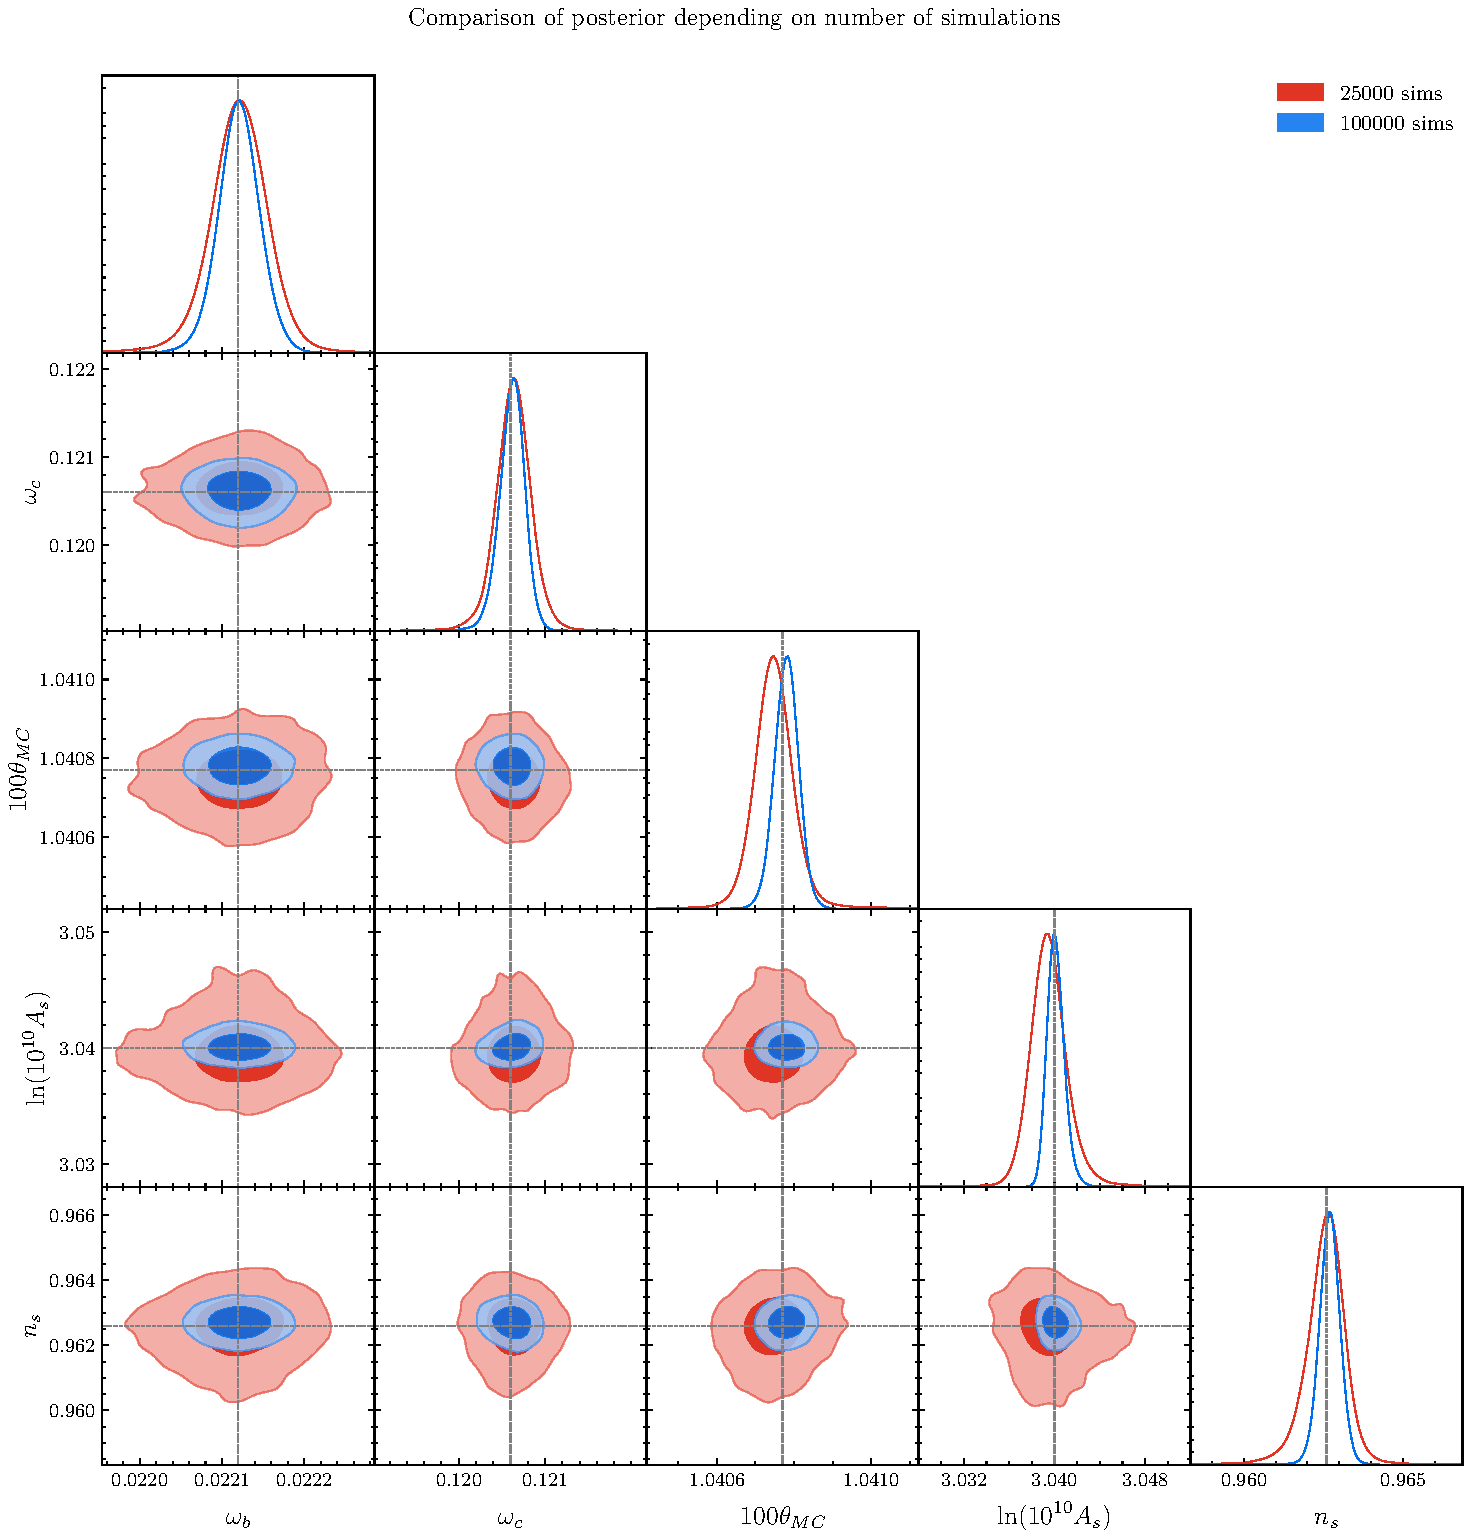
\includegraphics[scale=0.35]{img/nsims_comparison.pdf}
    \caption{PPC diagnostic of the inference performed with 25,000 and 100,000 training simulations of the $C_{\ell}^{TT}$ power spectrum. Both models were trained with the NPSE architecture. The dashed line shows the true value of the parameters. The model trained with 100,000 simulations exhibits better convergence than the one trained with 25,000 simulations, with a more concentrated distribution and smoother boundaries.}
    \label{fig:nsims_comparison}
\end{figure}

\begin{figure}
    \centering
    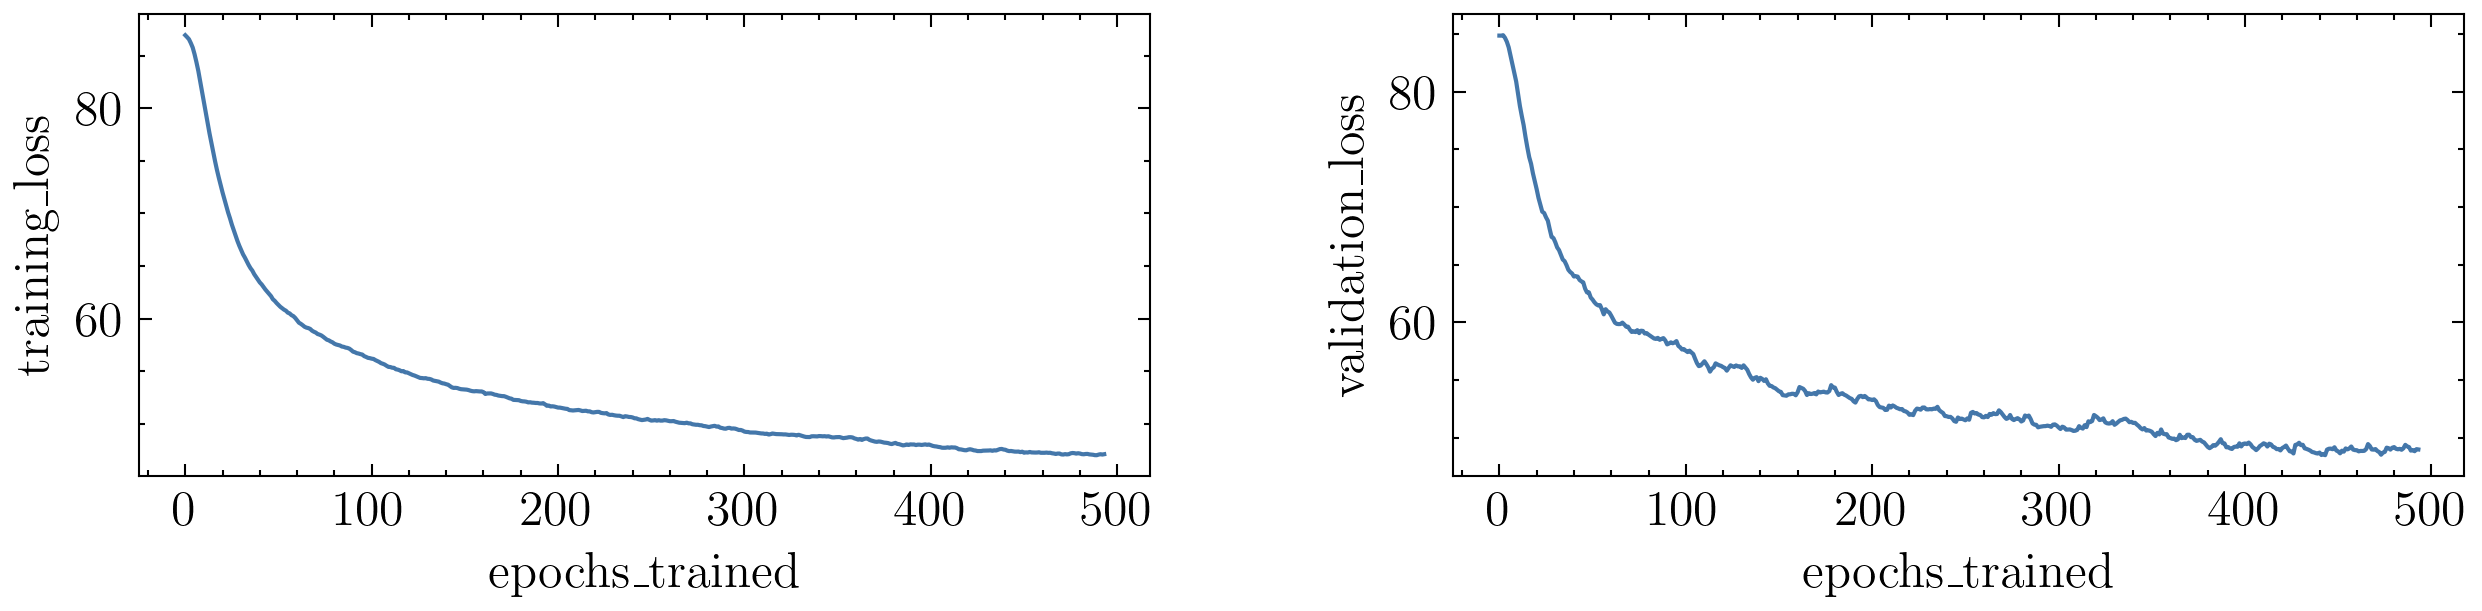
\includegraphics[scale=0.45]{img/NPSE_TT_tau_100000}
    \caption{Evolution of the loss function on training and validation sets across 500 epochs. The NPSE model was trained with 100,000 simulations of the $C_{\ell}^{TT}$ spectrum.}
    \label{fig:nsims_comparison}
\end{figure}

\begin{figure}
    \centering
    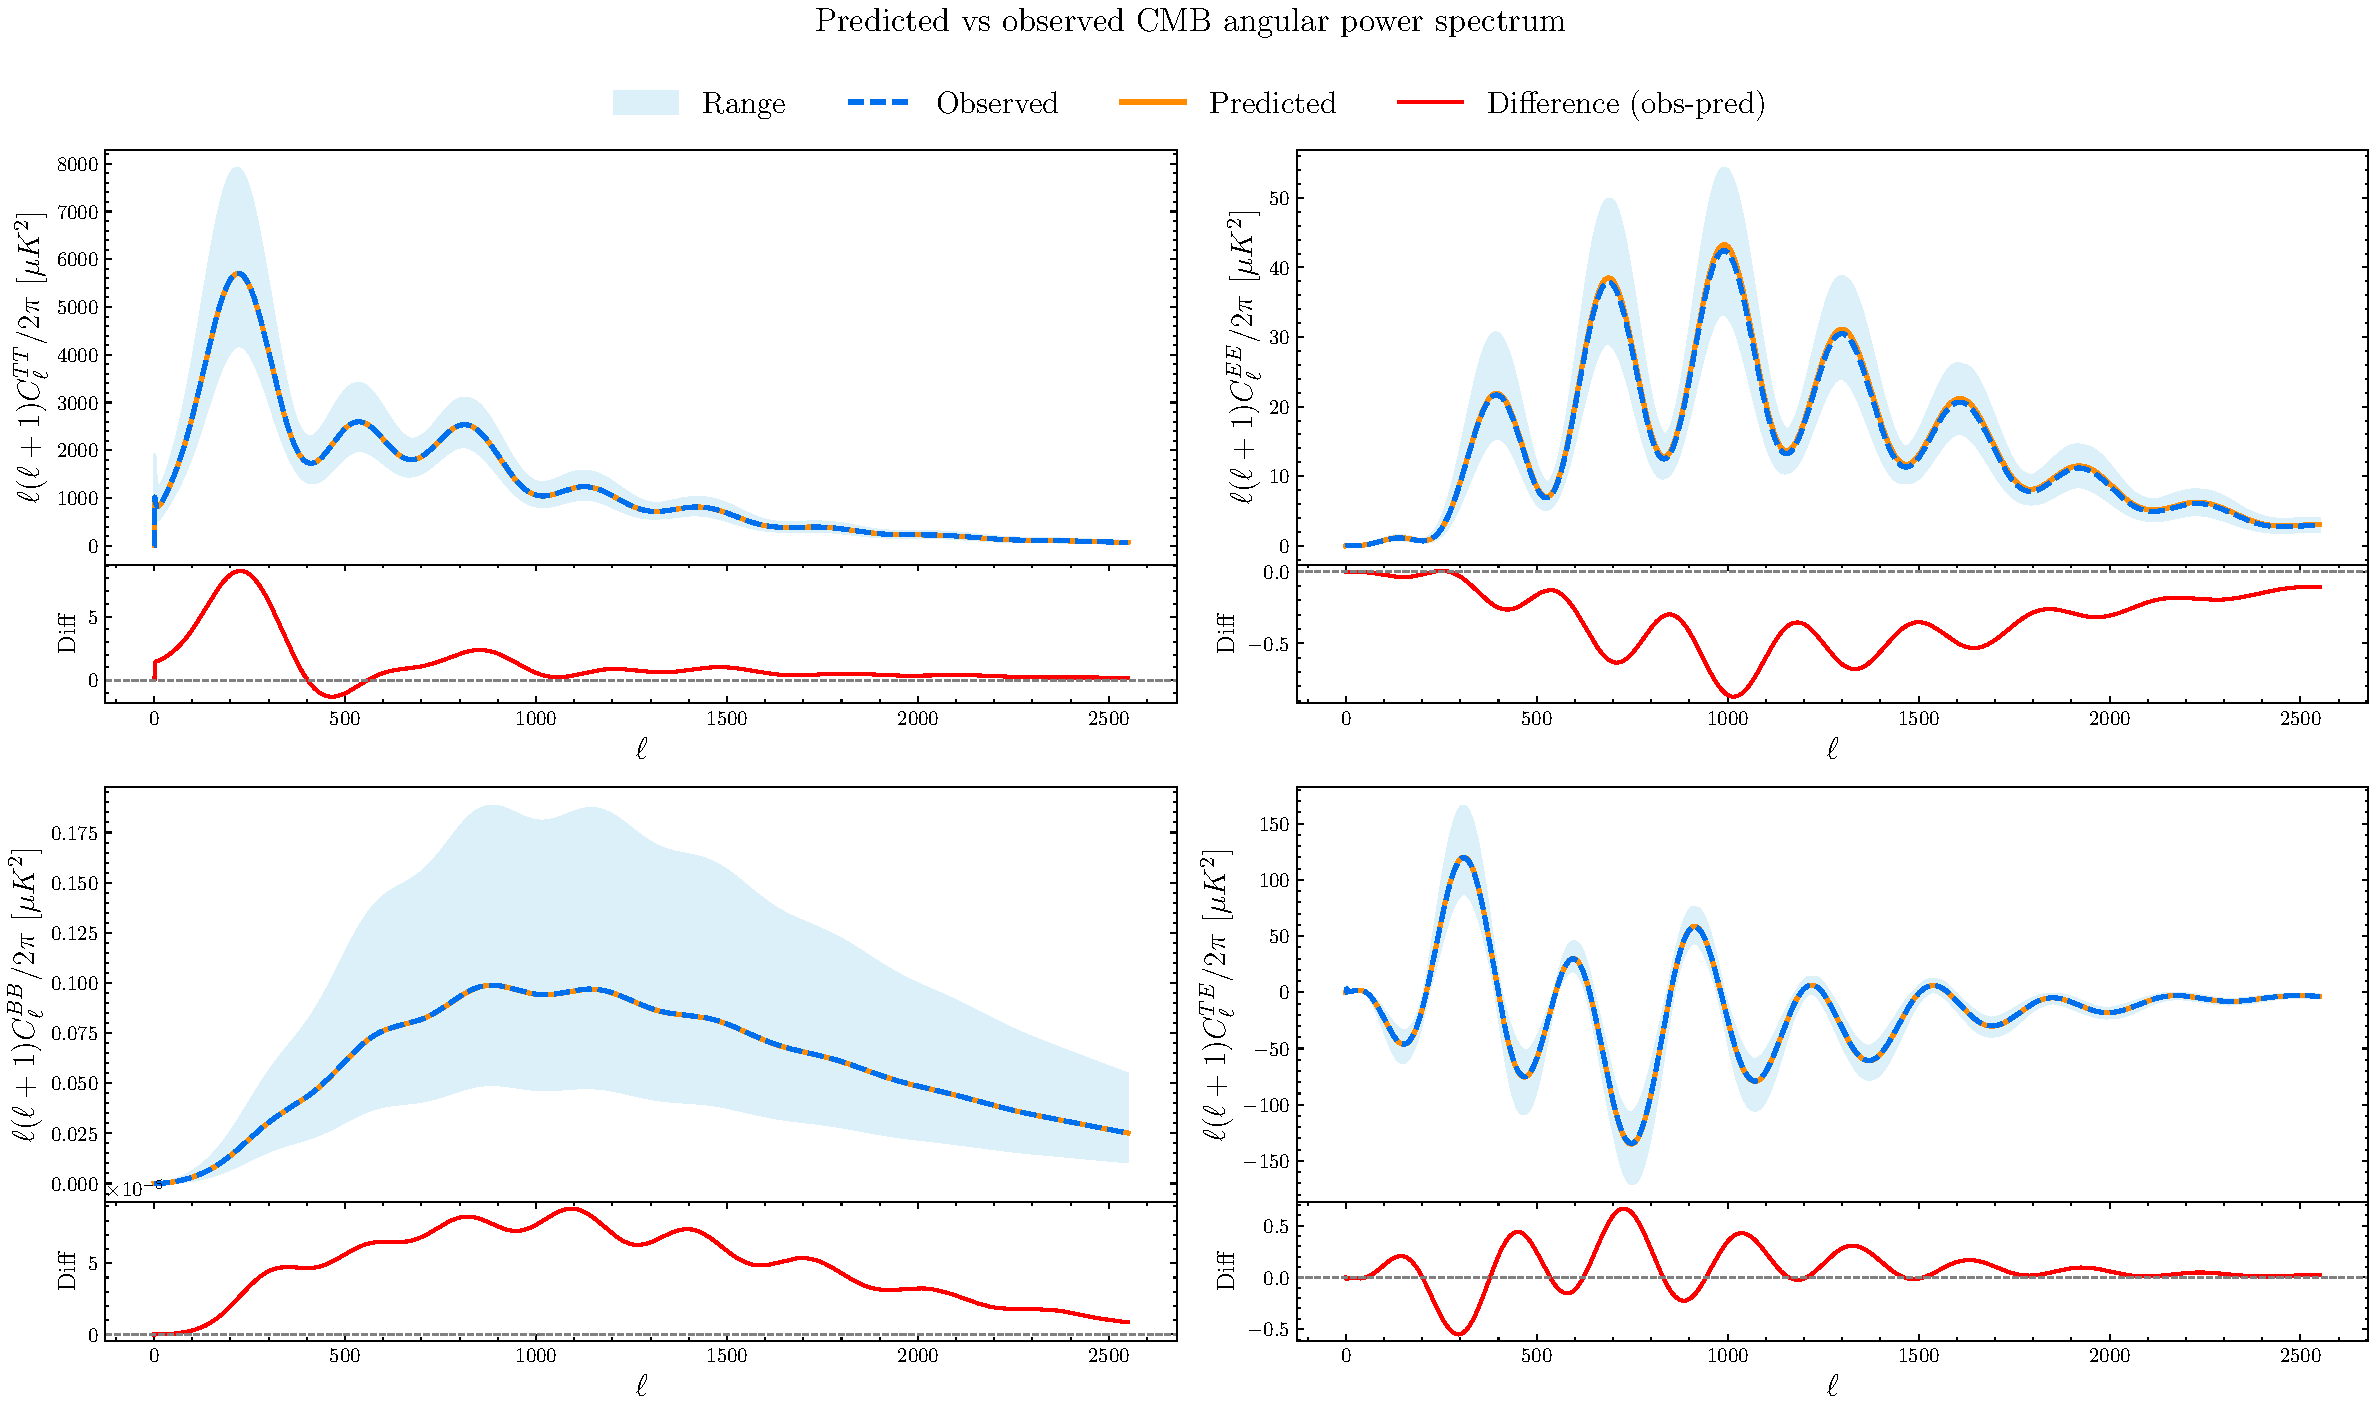
\includegraphics[scale=0.225]{img/cmb_aps_pred_vs_obs_0.pdf}
    \caption{Comparison of the power spectra $C_{\ell}^{TT}$, $C_{\ell}^{EE}$, $C_{\ell}^{BB}$, and $C_{\ell}^{TE}$ simulated with the true parameter values and the power spectra obtained from a random posterior sample derived from training an NPSE inference model with 100,000 simulations of the $C_{\ell}^{TT}$ power spectrum. The lower panel of each subplot shows the difference between the observed and predicted power spectra.} 
    \label{fig:pred_vs_obs}
\end{figure}

\begin{figure}
    \centering
    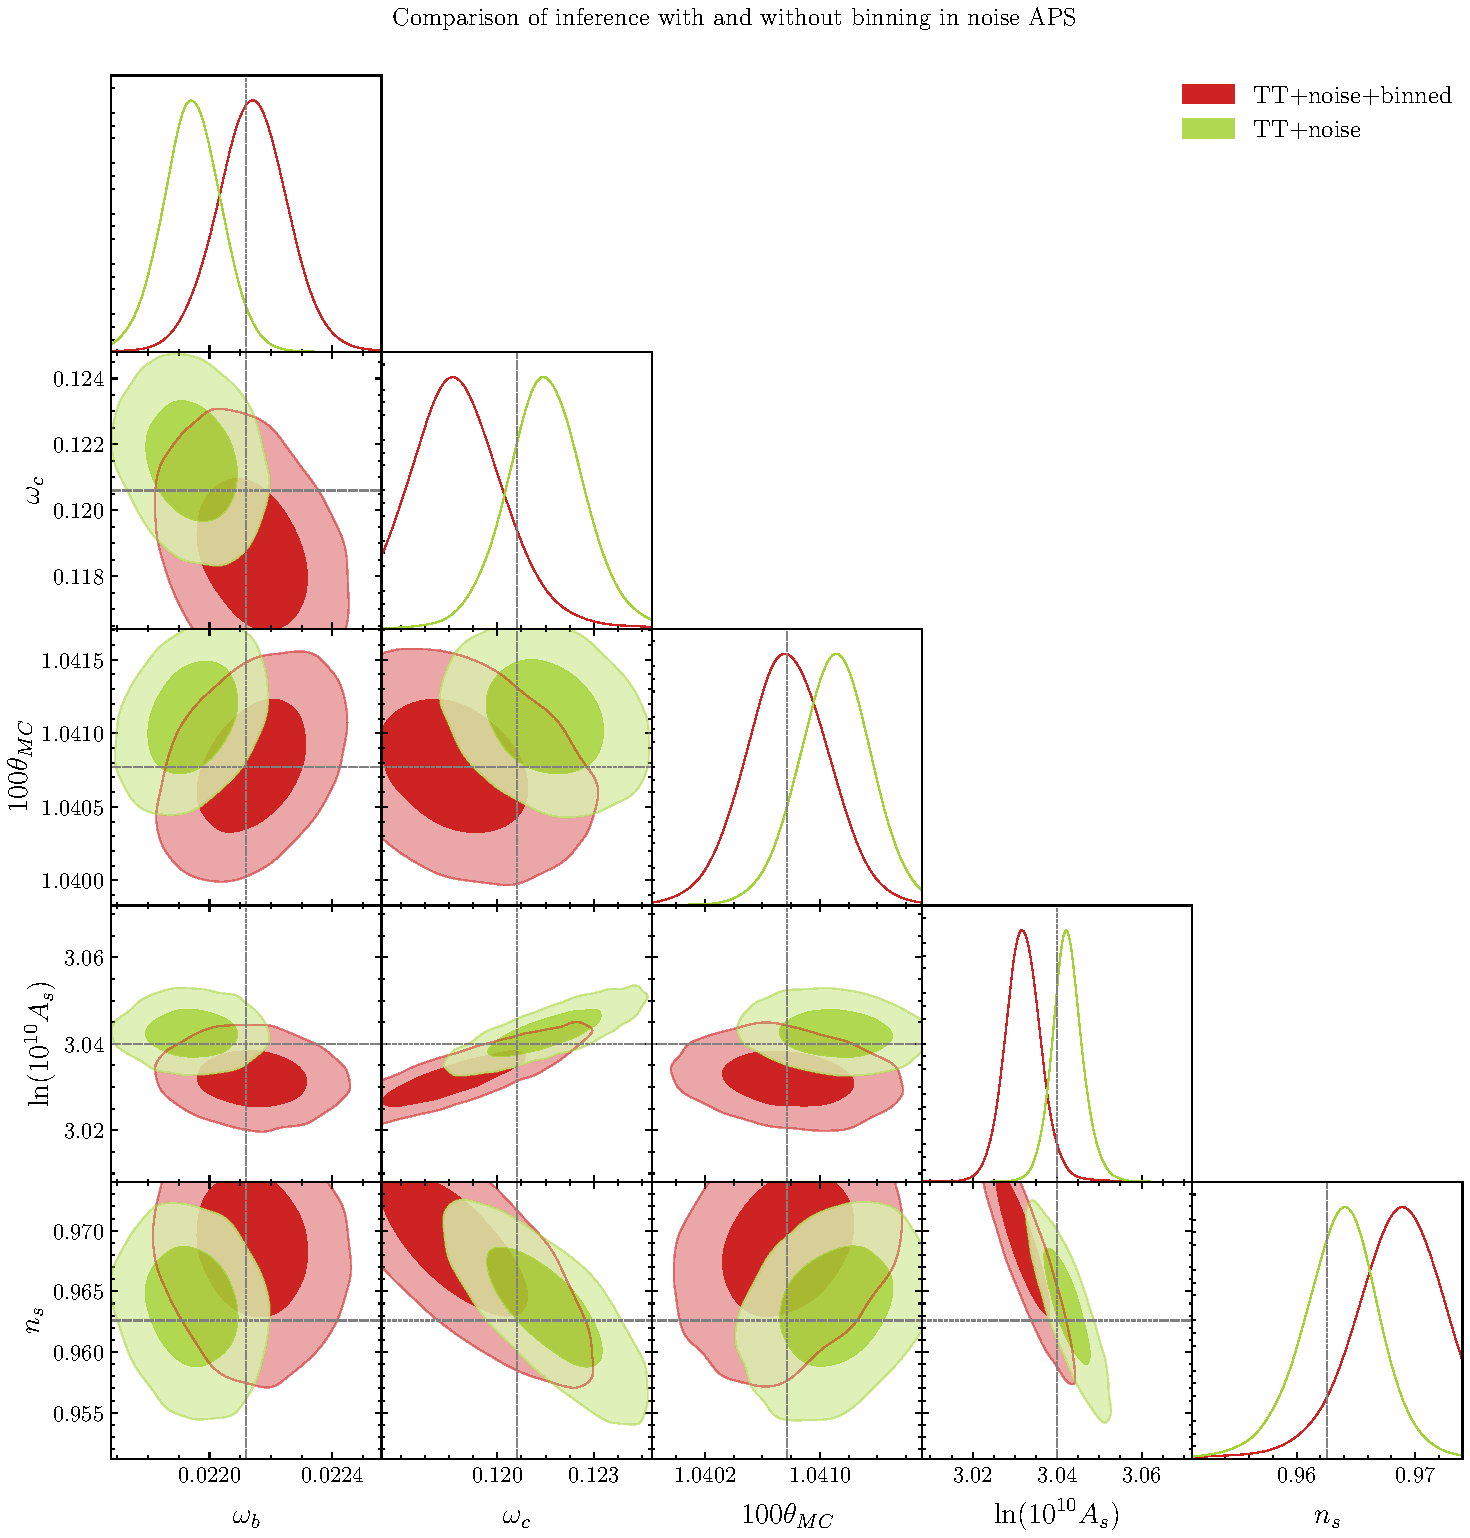
\includegraphics[scale=0.35]{img/inference_with_noise.pdf}
    \caption{Comparison of cosmological inference from the TT power spectrum, considering two training schemes: with unbinned noise (\texttt{TT+noise}) 
    and with noise averaged over 500 bins (\texttt{TT+noise+binned}).}
    \label{fig:nsims_comparison}
\end{figure}